\section{Geolog\'ia}
En la cuenca hidrogr\'afica de la quebrada La Linda se encuentran 2 unidades geol\'ogicas, una sedimentaria la cual corresponde al Miembro Urrao de la Fm. Penderisco y aguas arriba de la Quebrada La Linda se encuentra el Batolito Farallones.\\

\textbf{Batolito Farallones.Tmcf}
Ubicado al Sur del Stock de Cerro plateado de formaci\'on y de formaci\'on contemporanea a este. El Batolito Farallones recibe su nombre por encontrarse lozalizado al Este de la Localidad de Farallones.
El Batolito Farallones de edad Mioceno presenta una aureola de contacto extensa (500m aprox), fuertemente fallada y plegada con los sedimentos cret\'acicos que lo rodean en su extremo norte. Su altura alcanza apr\'oximadamente los 3400msnm exhibiendo escarpes casi totalmente verticales.
Su clasificaci\'on se determin\'o como intrusivo monzonitico, datado por el m\'etodo $K/Ar$ como originado hace 11 +- 2 m.a. \cite{farallones}
 

\textbf{Fm. Penderisco Miembro Urrao. Ksaau}
La sedimentaci\'on de la formaci\'on penderisco se ubica entre el cretaceo temprano a tardio como producto de flujos de turbiedad.
Est\'a compuesta por estratos de rocas que var\'ian en calibre desde areniscas pasando por limolitas y lodolitas (siendo esta la facie predominante) hasta chert, este \'ultimo se presenta frecuentemente como interestratificaciones finas. Se presentan igualmente conglomerados de tama\~no de clasto altamente variable (polim\'ictico), los cuales presentan espesores y arreglos altamente variables.
Tanto algunas lodolitas como estratos de areniscas exhiben estructuras de polaridad como estratificaci\'on cruzada.
Debido al emplazamiento de los intrusivos del Miocenos, los sedimentos de la Fm. Penderisco exhiben fuertes buzamientos que fluctuan  entre 60 y 70 grados. \cite{urrao}
Su estructura fue fuertemente modificada por el emplazamiento del Batolito Farallones en en Ne\'ogeno temprano. En la figura \ref{fig:mapageo}

\textbf{Fm. Barroso. Kvb}
En la zona de trabajo se presenta en un punto aislado sobre la via que de Ciudad Bolivar conduce a Quibdo.
All\'i ocurrencia es en forma de diabasa altamante fracturada \cite{barroso}, aunque no se pudo apreciar las intercalaciones de chert que describe la bibliograf\'ia consultada.

La descripci\'on geol\'ogica retomada de la informaci\'on bibliogr\'afica oficial sirvi\'o en los ensayos preliminares del software Scoops3D como referencia para seleccionar los par\'ametros de resistencia a usar en dichos ensayos.

\begin{figure}[H]
\centering
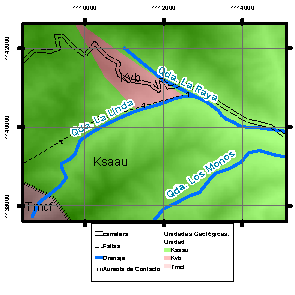
\includegraphics[scale=3]{img/geologia.pdf}
\caption{Mapa geol\'ogico de la zona de estudio basado en \cite{geol}. Acercamiento de elaboraci\'on propial.   }
\label{fig:mapageo}
\end{figure}


